
\chapter{الدراسة المرجعية}
بات من الواضح أن الدورات الاقتصادية هي ظاهرة حاكمة وملازمة للنشاط الاقتصادي. فمن المستحيل تحقيق النمو الاقتصادي بشكل مستقيم دون وجود تقلبات موجية متمثلة بحالات
انتعاش وازدهار وأخرى متمثلة بحالات ركود وكساد. بفهمنا لأسباب نشوء هذه الدورات وآلية التقلبات التي تحدث فيها
\parencite{10:mvcp}
وما ينتج عنها \cite{1:misp}، يمكننا بالتنبؤ بها واتخاذ القرارات المناسبة للحد
من حدّة هذه التقلبات.  \cite{wolfram:mvc}

أو القيام بالنشاطات واتخاذ القرارات والأخذ بالاحتياطات المناسبة التي تسمح بالخروج من حالات الانحطاط وزيادة مدّة حالات الازدهار والتوسع.
فكما رأينا في الفقرة \ref{sec:manage} يمكن للحكومات والبنوك المركزية التأثير على تقلبات الدورة الاقتصادية، وكلما كانت هذه التأثيرات استباقية، كلما قلّت حدّة التقلبات
وزادت السيطرة على الدورة الاقتصادية.
أيضاً نرى أنه من المهم على مدراء الشركات معرفة وتحليل الوضع الحالي للاقتصاد؛ أي تحديد المرحلة الحالية لدورة الاقتصاد التي تحكم السوق. فهذا سيساعدهم لاتخاذ القرار
سواء لزيادة كميات العرض، أو سحبها من السوق، زيادة التوظيف في الشركة، تصغير حجم الشركة، زيادة الاستثمار وتحريك رأس المال الثابت، تجميد السيولة أو تحريكها.

\section{مفهوم الدورة الاقتصادية}
يشير التاريخ إلى أنّ تطور النشاط الاقتصادي لا يتم بشكل خطي، إذ يعاني من تقلبات عديدة، تتعاقب فيها فترات من الازدهار وفترات من الانحطاط.
نسمي هذه الظاهرة بـالدورة الاقتصادية، وتعد ظاهرة ملازمة للنشاط الاقتصادي منذ القدم، وتندرج دراستها تحت الاقتصاد الكلي.

تعرّف الدورة الاقتصادية \LR{economic cycle} 
(أيضاً تسمى بدورة العمل \LR{business cycle} او دورة التجارة \LR{trade cycle}) 
بأنها التغيرات التي تحدث بشكل دوري في المؤشرات الاقتصادية 
مثل البطالة والتضخم وإجمالي الناتج المحلي حول خط نموها على المدى الطويل.

تحدث الدورات الاقتصادية بشكل ظاهر ومؤثر في الاقتصادات التي تتبع نهج السوق الحر أو الاقتصادات الرأسمالية،
وتحدث الدورة الاقتصادية على أربعة مراحل أساسية
(انظر الشكل \ref{fig:trend}) وهي:
\begin{enumerate}
	\item 
	مرحلة التوسع أو الانتعاش \LR{Expansion or Recovery} :
	تتسم هذه المرحلة بميل المستوى العام للأسعار إلى الثبات،
	أما النشاط الاقتصادي في مجموعه فيتزايد ببطء، وينخفض سعر الفائدة ، 
	ويتضائل المخزون السلعي، و تتزايد الطلبات على المنتجين لتعويض ما تم استنفاذه من هذا المخزون.
	\item 
	مرحلة الرواج أو القمة \LR{Peak or Boom}:
	تتسم هذه المرحلة بارتفاع مطرد في الأسعار،  وتزايد حجم الإنتاج الكلى بمعدل سريع، 
	وتزايد حجم الدخل ومستوى التوظيف%
	\footnote{
		يقصد بالتوظيف هنا توظيف عناصر الإنتاج وعوامله وليس المفهوم الضيق الذي يعني توظيف عنصر العمل فقط.
	}
	وتسعى البنوك المركزية حينها لرفع أسعار الفائدة وبيع السندات الحكومية لكبح جماح التضخم وسحب الفائض النقدي من الاقتصاد.
	\item 
	مرحلة الأزمة أو الركود \LR{Recession or Crisis}:
	وتسم هذه المرحلة بهبوط المستوى العام للأسعار، وتراجع إجمالي الناتج المحلى،
	وينتشر الذعر التجاري، وتطلب البنوك قروضها من العملاء، وتتزايد البطالة لتصل إلى أقصاها، كما يتزايد المخزون السلعى.
	\item 
	مرحلة الكساد أو القاع \LR{Trough or Depression}:
	تتسم بانخفاض الأسعار، وانتشار البطالة، وكساد التجارة.
	تسعى البنوك المركزية في هذه المرحلة لتخفيض سعر الفائدة لمستويات تقارب 0\% وشراء السندات الحكومية
	بهدف تشجيع الاستثمار لخفض مستوى البطالة إلى القيمة المستهدفة.
	هذه المرحلة هي الأخطر في الدورة الاقتصادية، وهي مرحلة ناتجة عن استمرار مرحلة الركود دون علاج صحيح.
	الخروج منها يحتاج إلى بذل عمل استثنائي، لانتشال وإخراج الاقتصاد من دائرة الكساد إلى مرحلة الانتعاش.
\end{enumerate}
تختلف مدة كل مرحلة عن الأخرى تبعاً للمعطيات وردود أفعال القوى الاقتصادية الأخرى في الاقتصاد،
ويتفق معظم الاقتصاديين على أن مدة الدورة الاقتصادية بداية من نقطة محددة ورجوعاً الى هذه النقطة مرة أخرى قد يتراوح من 3 سنوات الى 10 سنوات.

\begin{figure}[htb]
	\centering
	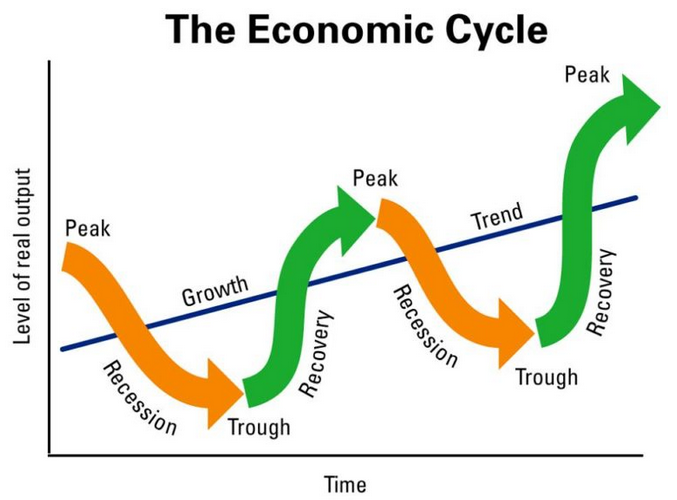
\includegraphics[width=0.7\linewidth]{images/trend.PNG}
	\caption{الدورة الاقتصادية ومراحلها الأربعة الأساسية}
	\label{fig:trend}
\end{figure}


\section{أشهر الدورات الاقتصادية}
يصنّف الاقتصاديون عادّة الدورات الاقتصادية إلى ثلاثة أنوع؛ الدورات	طويلة الأجل، والدورات متوسطة الأجل، والدورات قصيرة الأجل.
نبيّن فيما يلي أربعاً من أشهر الدورات الاقتصادية وسمات كل منها.
\subsection{دورة كتشن \LR{Kitchin cycle}}
دورة اقتصادية قصيرة الأجل، تمتد من 3 إلى 5 سنوات،
اكتشفها \LR{Joseph Kitchin} عام 1920.
تحدث هذه الدورة بسبب الفترات الزمنية المستغرقة لانتقال المعلومات
الاقتصادية والتي تؤثر على اتخاذ القرار في الشركات.
تقوم الشركات بالرد على تحسّن الوضع التجاري بزيادة كمية العرض
من خلال التوظيف الكامل لما تملكه من رأس مال.
نتيجة ذلك، خلال فترة زمنية تترواح من عدّة أشهر إلى سنتين،
يفيض السوق بالسلع. ثمّ يبدأ الطلب بالتناقص وتنخفض الأسعار،
ويتم تجميع هذه السلع في المخزونات، فتقوم الشركات بتخفيض
كمية العرض. تحتاج هذه العملية لفترة زمنية؛ انتقال معلومة
كون السوق فائض بالسلع يحتاج وقت، بالإضافة إلى الوقت الذي
تحتاجه الشركات لتأكيد هذه المعلومة واتخاذ القرار المناسب.

\subsection{دورة جوغلر \LR{Juglar cycle}}
تسمى أيضاً بدورة 
الاستثمار الثابت \LR{fixed investment cycle}، 
تتراوح مدتها من 7 إلى 11 عام.
اكتشفت من قبل \LR{Clement Juglar} عام 1862.
نلاحظ في دورة جوغلر تأرجح الاستثمار في
رأس المال الثابت \LR{fixed capital} وليس فقط التغييرات
في توظيفه كما هي الحالة في دورة كتشن.
أثبتت دراسة علمية عام 2010 بأن دورة جوغلر موجودة
في حركة إجمالي الناتج المحلي العالمي.



\subsection{دورة كوزنيت \LR{Kuznets cycle}}
دورة اقتصادية متوسطة الأجل تمتد من 15 إلى 25 عام.
اكتشفت من قبل \LR{Simon Kuznets} عام 1930.
قام كوزنيت بربط التغيرات في هذه الدورة مع الأحداث الديموغرافية،
وعلى وجه الخصوص، هجرة الداخل والخارج 
والتغييرات الكثيفة في البنى التحتية التي تحدث بسببها.
ولهذا سمّيت هذه الدورة أيضاً بدورة البناء \LR{building cycle}.


